\documentclass{beamer}


% ****************** Packages ******************
\usepackage[french]{babel}
\usepackage[T1]{fontenc}
\usepackage[utf8]{inputenc}
\usepackage{tikz}
\usepackage{graphicx}
\usepackage{caption}
\captionsetup[figure]{labelformat=empty} 
\usetheme{Madrid}
\setbeamertemplate{navigation symbols}{}%remove navigation symbols
\begin{document}
\date{12 mai 2015}

\begin{frame}
\frametitle{Slides pour les questions}
\end{frame}

\begin{frame}
	\frametitle{Octava}

	\begin{minipage}{0.35\linewidth}
             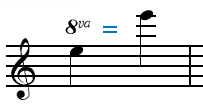
\includegraphics[width=4cm]{images/octava.png}
        \end{minipage}\hfill
        \begin{minipage}{0.6\linewidth}
             Notation octava affichée :
             \begin{itemize}
 	          \item À partir du mi (inclus) trois lignes au dessus de la portée
                  \item À partir de la frette 12, corde 1
                                         \item À partir de la frette 13, toutes les autres cordes
       	     \end{itemize}
         \end{minipage}

\bigbreak
	\begin{minipage}{0.35\linewidth}
             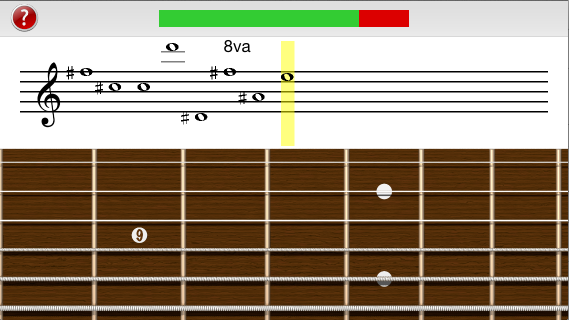
\includegraphics[width=4cm]{images/portee_frette_12.png}
                  \end{minipage}\hfill
                  \begin{minipage}{0.6\linewidth}
                       \begin{itemize}
                            \item Notes octaviées et notes non octaviées qui se côtoient autour de la frette 12
			    \item Petit écran : les notes aiguës superposent la notation 8va
                            \item Solution : biaiser l'aléatoire
                        \end{itemize}
                   \end{minipage}

\end{frame} 

\begin{frame}
	\frametitle{Octava : fausse note}

	\begin{block}{Sur la partie octaviée}
  	Comment afficher la fausse note entrée par l'utilisateur si elle est non octaviée ?
	\end{block}

	\begin{block}{Sur la partie non octaviée}
  	Comment afficher la fausse note entrée par l'utilisateur si elle est octaviée ?
	\end{block}


	\begin{block}{Problème}
	  Comment montrer qu'on sort ou qu'on rentre en octava clairement avec les contraintes :
	\begin{itemize}
		\item L'écran est petit : superposition des notes sur l'octava
		\item La portée doit restée facile à lire et à comprendre
	\end{itemize}
	\end{block}
\end{frame}

\begin{frame}
	\frametitle{Octava : fausse note}

	\begin{minipage}{0.35\linewidth}
             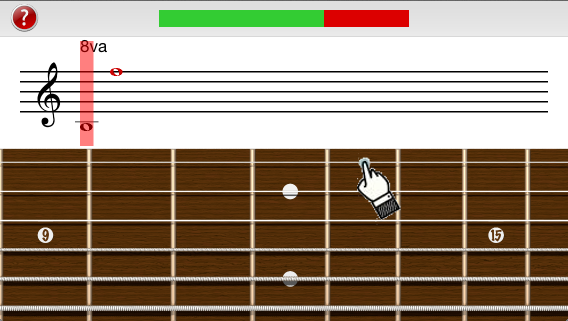
\includegraphics[width=4cm]{images/portee_deux_octava.png}
        \end{minipage}\hfill
           \begin{minipage}{0.6\linewidth}
		Si la note question et la note réponse nécessitent l'octava :
                 \begin{itemize}
                      \item Surbrillance rouge
                      \item Son de la fausse note
		      \item Fausse note affichée
                 \end{itemize}
         \end{minipage}
\bigbreak

	\begin{minipage}{0.35\linewidth}
             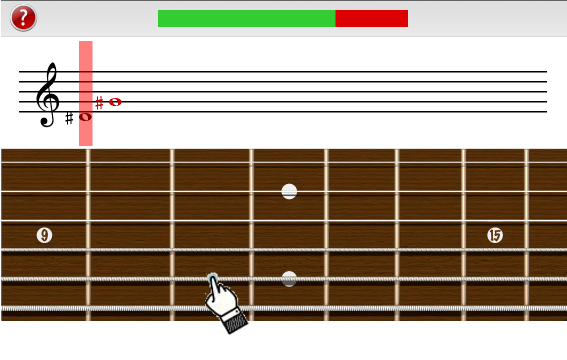
\includegraphics[width=4cm]{images/portee_octava_tap2.png}
       \end{minipage}\hfill
              \begin{minipage}{0.6\linewidth}
			Si la note question et la note réponse ne nécessitent pas l'octava :
                 \begin{itemize}
                     \item Surbrillance rouge
                     \item Son de la fausse note
		    \item Fausse note affichée
             \end{itemize}
         \end{minipage}
\end{frame} 

\begin{frame}
	\frametitle{Octava : fausse note}

	\begin{minipage}{0.35\linewidth}
             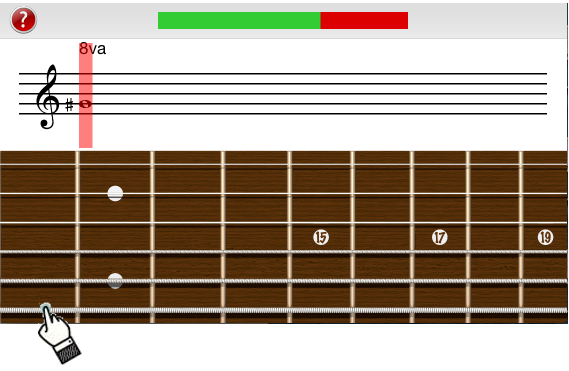
\includegraphics[width=4cm]{images/portee_octava_tap.png}
         \end{minipage}\hfill
             \begin{minipage}{0.6\linewidth}
			Si l'activation de l'octava diffère pour la note question et la note réponse : 
               \begin{itemize}
                    \item Surbrillance rouge
                    \item Son de la fausse note
	            \item Si la fausse note peut être octaviée :
                \begin{itemize}
                  \item Fausse note affichée
                 \item Sinon, fausse note non affichée
              \end{itemize}
                \end{itemize}
                \end{itemize}
            \end{minipage}

\end{frame} 

\end{document}
